\documentclass{beamer}
\usetheme[nat]{Frederiksberg}

\usepackage{algorithm}
\usepackage[noend]{algorithmic}
\usepackage{adjustbox}
\usepackage{multirow}
\usepackage{longtable}
\usepackage{siunitx}
\usepackage{amsmath}

\begin{document}
\title{Bachelor's thesis defense}
\author{Nikolaj Dybdahl Rathcke}
\date{June 18, 2015}

\frame{\titlepage}

\section{Background}
\frame{\frametitle{Background}

\begin{columns}[c]

\column{4cm}
\begin{itemize}
\item Inexpensive sequencing data
\item Centroid-based clustering
\item What does \texttt{klust} solve?
\end{itemize}

\column{8cm}
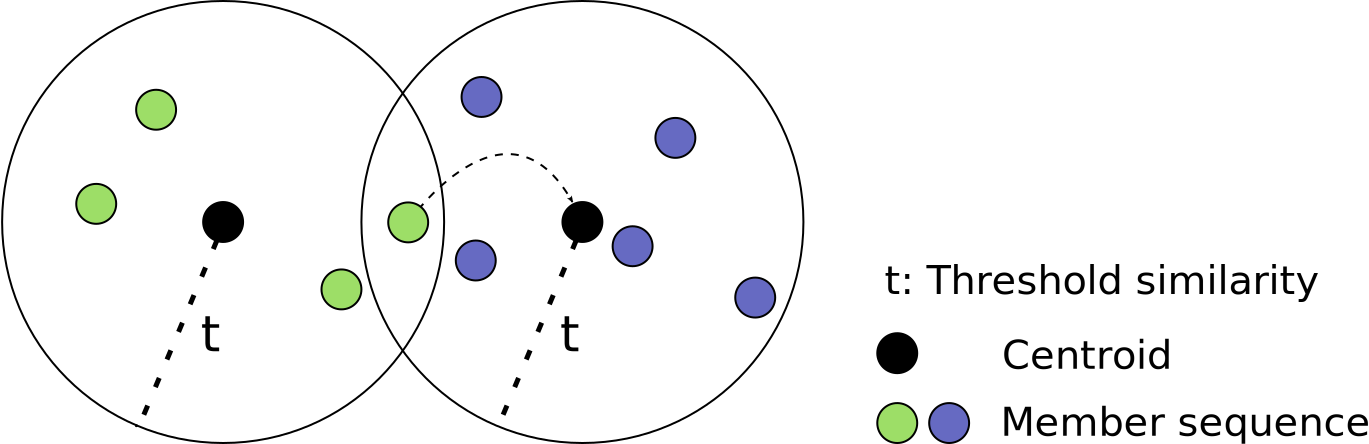
\includegraphics[width=\textwidth]{graphics/Clustering.pdf}

\end{columns}

}


\section{Distance metric}
\frame{\frametitle{Distance metric}
\begin{columns}[c]

\column{5cm}
\begin{itemize}
\item Sequence alignment is expensive
\item $k$-mer is cheap to compute
\item The Manhattan distance
\end{itemize}

\column{5cm}
\begin{itemize}
\item Windows ensures that string of different length are still comparable
\item \textsc{K-Dist}
\end{itemize}
\end{columns}
\vfill
\includegraphics[width=\textwidth]{graphics/freq_vecs.pdf}
}

\frame{\frametitle{\textsc{K-Dist} example with $k=2$}
\includegraphics<1>[width=\textwidth]{graphics/K_Dist_1.pdf}
\includegraphics<2>[width=\textwidth]{graphics/K_Dist_2.pdf}
\includegraphics<3>[width=\textwidth]{graphics/K_Dist_3.pdf}
}

\section{Clustering algorithm}
\frame{\frametitle{Clustering algorithm}
\begin{itemize}
\item Greedy algorithm improves time complexity
\end{itemize}
\vfill
\begin{center}
\includegraphics[scale=0.4]{graphics/Greedy_Clustering.pdf}
\end{center}
}

\frame{\frametitle{Clustering algorithm}
\begin{itemize}
\item Greedy algorithm improves time complexity
\item Intersection criterion to quickly dismiss sequences that are not likely to belong to a cluster
\end{itemize}
\begin{block}{Intersection criterion}
$|K(s)\cap K(c)| \geq |K(c)|\cdot id$
\end{block}
\vfill
\includegraphics<1>[width=\textwidth]{graphics/freq_vecs.pdf}
\includegraphics<2>[width=\textwidth]{graphics/Kmer_set_vecs.pdf}

}

\frame{\frametitle{Clustering algorithm}
\begin{itemize}
\item Greedy algorithm improves time complexity
\item Intersection criteria to quickly dismiss sequences that are not likely to belong to a cluster
\item Ordering centroids can improve performance \pause
\item The centroid structure \pause
\item \textsc{K-Clust}
\end{itemize}
}

% \frame{\frametitle{\textsc{K-Clust}}
% \begin{algorithm}[H]
% \begin{algorithmic}[1]
% \REQUIRE{S,C,$k$,$id$,$max\_rejects$}
% \FORALL{$s\in S$}
% \FORALL{$c\in C$}
% \IF{Intersection criteria $\land$ $rejects \neq max\_rejects$}
% \IF{Distance above threshold}
% \STATE{Assign $s$ to cluster represented by $c$}
% \STATE{Move $c$ to the front of the list and \texttt{break}}
% \ENDIF
% \IF{Distance above threshold to $c\to link$}
% \STATE{Assign $s$ to cluster represented by $c\to link$}
% \STATE{Move $c\to link$ to the front of the list and \texttt{break}}
% \ENDIF
% \ENDIF
% \STATE{+{}+$rejects$} and set link if there is one.
% \ENDFOR
% \STATE Make a new cluster represented by $s$
% \ENDFOR
% \end{algorithmic}
% \caption{\textsc{K-Clust} algorithm}
% \label{alg:K-Clust}
% \end{algorithm}
% }


\frame{\frametitle{\textsc{K-Clust}}
\includegraphics<1>[width=\textwidth]{graphics/K_Clust_1.pdf}
\includegraphics<2>[width=\textwidth]{graphics/K_Clust_2.pdf}
\includegraphics<3>[width=\textwidth]{graphics/K_Clust_3.pdf}
\includegraphics<4>[width=\textwidth]{graphics/K_Clust_4.pdf}
\includegraphics<5>[width=\textwidth]{graphics/K_Clust_5.pdf}
\includegraphics<6>[width=\textwidth]{graphics/K_Clust_6.pdf}
\includegraphics<7>[width=\textwidth]{graphics/K_Clust_7.pdf}
\includegraphics<8>[width=\textwidth]{graphics/K_Clust_8.pdf}
\includegraphics<9>[width=\textwidth]{graphics/K_Clust_9.pdf}
\includegraphics<10>[width=\textwidth]{graphics/K_Clust_10.pdf}
\includegraphics<11>[width=\textwidth]{graphics/K_Clust_11.pdf}
\includegraphics<12>[width=\textwidth]{graphics/K_Clust_12.pdf}
\includegraphics<13>[width=\textwidth]{graphics/K_Clust_13.pdf}
\includegraphics<14>[width=\textwidth]{graphics/K_Clust_14.pdf}
\includegraphics<15>[width=\textwidth]{graphics/K_Clust_15.pdf}
\includegraphics<16>[width=\textwidth]{graphics/K_Clust_16.pdf}
\includegraphics<17>[width=\textwidth]{graphics/K_Clust_17.pdf}
\includegraphics<18>[width=\textwidth]{graphics/K_Clust_18.pdf}
\includegraphics<19>[width=\textwidth]{graphics/K_Clust_19.pdf}
\includegraphics<20>[width=\textwidth]{graphics/K_Clust_20.pdf}
\includegraphics<21>[width=\textwidth]{graphics/K_Clust_21.pdf}
\includegraphics<22>[width=\textwidth]{graphics/K_Clust_22.pdf}
\includegraphics<23>[width=\textwidth]{graphics/K_Clust_23.pdf}
\includegraphics<24>[width=\textwidth]{graphics/K_Clust_24.pdf}
\includegraphics<25>[width=\textwidth]{graphics/K_Clust_25.pdf}
\includegraphics<26>[width=\textwidth]{graphics/K_Clust_26.pdf}
}

\section{Results}
\frame{\frametitle{Results}
\begin{itemize}
\item Evaluation of \textsc{K-Clust} with synthetic data
\item Evaluation of \texttt{klust} on real data
\end{itemize}
}

\frame{\frametitle{Multi-dimensional scaling of clustering output from \texttt{SILVA}}
Clustering on $40$ very different sequences with $9$ copies of each that has been altered.
\begin{center}
\includegraphics[scale=0.38]{graphics/MDS_Synthetic.pdf}
\end{center}
}

\frame{\frametitle{Comparison of \texttt{klust} and \texttt{USEARCH} on \texttt{RDP}}
\begin{table}
  \scriptsize
  \begin{adjustbox}{center}
  \begin{tabular}{c|r|r|r|lr|l}
  \multirow{2}{*}{}
  Clustering & \multicolumn{1}{c|}{Time} & \multicolumn{1}{c|}{Throughput} & \multicolumn{1}{c|}{Clusters} & \multicolumn{2}{c|}{Cluster sizes}& \multicolumn{1}{c}{Max} \\
  algorithm & \multicolumn{1}{c|}{(sec.)} & \multicolumn{1}{c|}{(seqs./sec.)} & & & & \multicolumn{1}{c}{memory} \\
  \hline \hline
  \multirow{3}{*}
  {}\textsc{K-Clust},  & & & & Max. & \num{100832} & \\
  $k=5, id=0.85, m=8,$ & \num{5420.8} & \num{557.10} & \num{220982} & Avg. & $13.67$ & $\approx\num{2031}$ MB\\
  incr. sort           & & & & Min. & $1$ & \\
  \hline
  \multirow{3}{*}
  {}\textsc{K-Clust},  & & & & Max. & \num{55992} & \\
  $k=5, id=0.9, m=8,$ & \num{11948.7} & \num{252.74} & \num{344122} & Avg. & $8.78$ & $\approx\num{2031}$ MB\\
  incr. sort           & & & & Min. & $1$ & \\
  \hline
  \multirow{3}{*}
  {}\texttt{USEARCH},        & & & & Max. & \num{65654} & \\
  $id=0.95,$ decr. sort      & \num{6874.0} & \num{439.20} & \num{261880} & Avg. & $11.50$ & $\approx\num{1433}$  MB \\
  \texttt{-cluster\_smallmem} & & & & Min. & $1$ & \\
  \hline
  \multirow{3}{*}
  {}\texttt{USEARCH},        & & & & Max. & \num{56279} & \\
  $id=0.97,$ decr. sort      & \num{11980.0} & \num{252.00} & \num{471982} & Avg. & $6.40$ & $\approx\num{2560}$  MB \\
  \texttt{-cluster\_smallmem} & & & & Min. & $1$ & \\
  \end{tabular}
  \end{adjustbox}
\end{table}
}


\section{Future work}
\frame{\frametitle{Future work}

\begin{itemize}
\item Link optimization effectively using max rejects \\
\item Optimizing distance metric to better recognize mutations \\
\item A better merge strategy for a solution using parallelization
\end{itemize}

}

\end{document}
